\documentclass{article}\usepackage[]{graphicx}\usepackage[]{color}
%% maxwidth is the original width if it is less than linewidth
%% otherwise use linewidth (to make sure the graphics do not exceed the margin)
\makeatletter
\def\maxwidth{ %
  \ifdim\Gin@nat@width>\linewidth
    \linewidth
  \else
    \Gin@nat@width
  \fi
}
\makeatother

\definecolor{fgcolor}{rgb}{0.345, 0.345, 0.345}
\newcommand{\hlnum}[1]{\textcolor[rgb]{0.686,0.059,0.569}{#1}}%
\newcommand{\hlstr}[1]{\textcolor[rgb]{0.192,0.494,0.8}{#1}}%
\newcommand{\hlcom}[1]{\textcolor[rgb]{0.678,0.584,0.686}{\textit{#1}}}%
\newcommand{\hlopt}[1]{\textcolor[rgb]{0,0,0}{#1}}%
\newcommand{\hlstd}[1]{\textcolor[rgb]{0.345,0.345,0.345}{#1}}%
\newcommand{\hlkwa}[1]{\textcolor[rgb]{0.161,0.373,0.58}{\textbf{#1}}}%
\newcommand{\hlkwb}[1]{\textcolor[rgb]{0.69,0.353,0.396}{#1}}%
\newcommand{\hlkwc}[1]{\textcolor[rgb]{0.333,0.667,0.333}{#1}}%
\newcommand{\hlkwd}[1]{\textcolor[rgb]{0.737,0.353,0.396}{\textbf{#1}}}%

\usepackage{framed}
\makeatletter
\newenvironment{kframe}{%
 \def\at@end@of@kframe{}%
 \ifinner\ifhmode%
  \def\at@end@of@kframe{\end{minipage}}%
  \begin{minipage}{\columnwidth}%
 \fi\fi%
 \def\FrameCommand##1{\hskip\@totalleftmargin \hskip-\fboxsep
 \colorbox{shadecolor}{##1}\hskip-\fboxsep
     % There is no \\@totalrightmargin, so:
     \hskip-\linewidth \hskip-\@totalleftmargin \hskip\columnwidth}%
 \MakeFramed {\advance\hsize-\width
   \@totalleftmargin\z@ \linewidth\hsize
   \@setminipage}}%
 {\par\unskip\endMakeFramed%
 \at@end@of@kframe}
\makeatother

\definecolor{shadecolor}{rgb}{.97, .97, .97}
\definecolor{messagecolor}{rgb}{0, 0, 0}
\definecolor{warningcolor}{rgb}{1, 0, 1}
\definecolor{errorcolor}{rgb}{1, 0, 0}
\newenvironment{knitrout}{}{} % an empty environment to be redefined in TeX

\usepackage{alltt}
\usepackage[margin=1.25in]{geometry}
\usepackage{graphicx, hyperref, float, multicol, pdflscape, enumerate, paralist}
\usepackage{amssymb,amsmath,amsthm} 
\usepackage[backend=bibtex, natbib=true]{biblatex}
\addbibresource{../references/references.bib}

\usepackage{color}
\newcommand{\ak}[1]{{\color{magenta} #1}}
\newcommand{\mj}[1]{{\color{blue} #1}}

\theoremstyle{plain}
\newtheorem{res}{Result}

\setlength{\parindent}{0cm}
\renewcommand{\baselinestretch}{1.5}

\title{Independence of Periodogram Ordinates at the Fourier Frequencies}
\author{Andee Kaplan \& Maggie Johnson}
\date{December 16, 2013}
\IfFileExists{upquote.sty}{\usepackage{upquote}}{}

\begin{document}

\maketitle



\section{Motivation}

To explore whether it is reasonable to estimate the spectral density of a stationary time series using Bayesian methods. To do this, it is necessary to rely on the asymptotic distributional properties of periodogram ordinates. The motivation behind this work is the following model.
\begin{align}
\label{eq:eqn1}
I_n(\omega_r) |f(\omega_r) &\stackrel{\cdot}{\sim}\text{ indep } \text{Exp}(2\pi f(\omega_r)) \\
\label{eq:eqn2}
f(\omega_r) & \sim \pi(\theta)\\
\label{eq:eqn3}
f(\omega_r) | I_n(\omega_r) &\propto 2\pi f(\omega_r) e^{-2\pi f(\omega_r) y} \pi(\theta)
\end{align}
The periodogram values at $\omega_r$ are only asymptotically distributed as independent exponentials, so to construct the Bayesian model it is essential that the asymptotic behavior in Equation \ref{eq:eqn1} holds. This research uses simulations to assess two results by Lahiri, which state conditions necessary for periodogram ordinates to be asymptotically independent \cite{lahiri2003necessary}.


\section{Background and Problem Statement}

Spectral analysis, or ``frequency domain analysis" is the analysis of stationary time series $\{X_t\}$ using the decomposition $\{X_t\}$ into sinusoidal componenets. Spectral analysis is equivalent to ``time domain" analysis based on the autocovariance function, but can be more useful in applications where sinusoidal behavior is relevant. The spectral density of a mean-zero stationary process $\{X_t\}$ is used to describe the frequency decomposition of the autocovariance function $\gamma(\cdot)$ and the process $\{X_t\}$ \cite{brockwell2002introduction}. It is the function $f(\cdot)$ defined by 
\begin{align}
f(\omega) = \frac{1}{2\pi} \sum_{h=-\infty}^{\infty} e^{-ih\omega} \gamma(h), \hspace{.5cm} -\infty < \omega < \infty
\end{align}
where $e^{i\omega}=\cos(\omega)+i\sin(\omega)$ and $i=sqrt(-1)$ \cite{brockwell2002introduction}. The periodogram, $I_n(\cdot)$ of $\{X_t\}$ can be regarded as a sample estimator of $2\pi f(\cdot)$ \cite{brockwell2002introduction}. The periodogram of $\{x_1,...,x_n\}$ at a frequencey $\omega$ is the function
\begin{align}
I_n(\omega) = \frac{1}{n} \left\lvert \sum_{t=1}^n x_t e^{-it\omega} \right\rvert^2
\end{align}

\begin{res} \label{res:first}
Let $f(\omega_r) \not= 0, 1 \le r \le k$ where $f$ denotes the spectral density of a stationary time series $\{X_t\}$. Then when $n\rightarrow \infty$ the joint distribution of the periodogram at $\omega_r$, $I_n(\omega_r)$, tends to that of $k$ mutually indepependent random variables distributed as $\text{Exponential}(2\pi f(\omega_r))$ for $0<\omega_r<\pi$ \cite{brockwell2002introduction}. 
\end{res}

Result~\ref{res:first} describes the asymptotic distribution of a periodogram at fixed frequencies. In practice, this result has often been used with the Fourier frequencies, $\{\omega_j = 2\pi j/n : j=1,...,n\}$, in a fixed time period. \cite{brockwell2002introduction}. However, it has been shown that the asymptotic behavior of the periodogram at the Fourier frequencies does not hold as $n \rightarrow \infty$ by SN Lahiri \cite{lahiri2003necessary}. In his paper, ``A necessary and sufficient condition for asymptotic independence of discrete Fourier transforms under short-and long-range dependence," Lahiri also derived two results that describe behavior required for a set of frequencies to satisfy the asymptotic independence assumption in result~\ref{res:first}.

\begin{res} \label{res:lahiri}
In the absense of data tapering,
\begin{enumerate}[(a)]
\item the periodogram values at asymptotically distant ordinates ($I_n(\omega_r)$) are asymptotically independent.  Asymptotically distant ordinates $\{\omega_{ln}\}, \{\omega_{kn}\}$ satisfy $|n(\omega_{ln} - \omega_{kn})| \rightarrow \infty$ as $n \rightarrow \infty$.

\item the periodogram values at asymptotically close ordinates which are asymptotically distant from the sequence $\{0\}$ are asymptotically independent. Asymptotically close ordinates $\{\omega_{ln}\}, \{\omega_{kn}\}$ satisfy $|n(\omega_{ln} - \omega_{kn})| \rightarrow 2\pi l$ for some nonzero integer $l$ as $n \rightarrow \infty$ \cite{lahiri2003necessary}.
\end{enumerate}
\end{res}

%Result~\ref{res:first} gives us the asymptotic distribution of a periodogram at fixed frequencies, while result~\ref{res:lahiri} details properties of frequencies that define where the independence holds. 

Results~\ref{res:first} and ~\ref{res:lahiri} lend to the question: ``Can a subset of sufficiently spaced and and distant from zero \textit{Fourier} frequencies be constructed such that the periodogram ordinates at these frequencies are asymptotically independent and exponentially distributed?" We explore these two results to determine if, for large $n$,
\begin{enumerate}
  \item result~\ref{res:first} will not, in fact, hold at the Fourier frequencies, and
  \item if (1) is true, a usable subset of Fourier frequencies can be constructed such that result~\ref{res:first} holds.
\end{enumerate}

%at at what point distant from zero and at what spacings close to zero do the approximate independence and exponential distribution fail in the periodogram values. 



\section{Models}\label{sec:models}

To explore the asymptotic behavior of the periodogram at the Fourier frequencies, we used ARMA time series models, as these are the only class of models with known spectral densities. A subset of the models considered are: \begin{inparaenum}[\itshape a\upshape)]
\item IID Gaussian(0, 1);
\item AR(1) with $\phi = 0.5$; 
\item AR(4) with $\boldsymbol{\phi} = [0.08, 0.33, 0.1, 0.45$];
\item MA(1) with $\theta = 0.7$; and
%\item MA(2) with $\boldsymbol{\theta} = [paste(model.ma2$ma, collapse=", ")$];
\item ARMA(4,1) with $\boldsymbol{\phi} = [0.08, 0.33, 0.1, 0.45$] and $\theta = 0.7$.
%\item ARMA(4,2) with $\boldsymbol{\phi} = [paste(model.arma42$ar, collapse=", ")$] and $\boldsymbol{\theta} = [paste(model.arma42$ma, collapse=", ")$].
\end{inparaenum}

\subsubsection*{IID Gaussian}
The following result about the IID Gaussian model provides knowledge of the exact, rather than asymptotic, behavior of the periodogram at any frequency.

\begin{res}
For $\{X_t\} \stackrel{\text{IID}}{\sim} \text{N}(0,\sigma^2)$, the periodogram values $\left\{ I_n(\omega_j): \omega_j \in \mathcal{F}_n, \omega_j \not\in \{0,\pi\} \right\}$ are IID Exponential($\sigma^2$) random variables \cite{brockwell2002introduction}.
\end{res}

This model was used as an initial baseline check to support the testing procedure of independent exponentially distributed ordinates. If our procedure showed failure with the IID Gaussian white noise model, then this would be an indication of an issue with the procedure, rather than the frequency spacings. The spectral density of the IID Gaussian model is $f_X(\omega) = \sigma^2/2\pi, \omega \in [-\pi, \pi]$.

\subsubsection*{ARMA(p,q)}
We exclusively used ARMA models as our experimental models because the spectral density of an ARMA model has a known and closed form. An ARMA model is a process $\{X_t\}$ with the form $\phi(B)X_t = \theta(B)Z_t$ where $B$ is the backshift operator and $\{Z_t\}$ is WN(0,$\sigma^2$). Models of this form have spectral density
\begin{align}
f_X(\omega) = \frac{\sigma^2}{2\pi} \frac{|\theta(e^{-i \omega})|^2}{|\phi(e^{-i \omega})|^2}, \omega \in [-\pi, \pi] \text{\cite{brockwell2002introduction}}.
\end{align}

%Without the exact knowledge of the spectral density function, we would not be able to test the distributions of the periodogram at each fequencies. \mj{mention moving window?}


\section{Methods}


For result~\ref{res:first} to hold for $\{X_t\}=\{x_1,...,x_n\}$ at the full Fourier frequencies, or a subset of Fourier frequencies, the joint asymptotic distribution of the periodogram ordinates $I_n(\omega)$ must be equivalent to the product of $n$ independent exponential distributions with means equal to $2\pi f(\omega)$. It is difficult to test the distribution of the full asymptotic joint distribution, so we split the problem into two parts: (1) a test of asymptotic exponential distribution at each $\omega_j, j=1,...,n$, and (2) a method to test independence over $\omega$. Independence is tested pairwise across all frequencies of interest. We implement the following testing procedure and repeat $s$ simulations of the tests to determine if the tests reject exponentiality and indepence at similar rates as the Type I errors of our tests ($\alpha$).
\paragraph{Procedure}
\begin{enumerate}
\item Simulate $M$ draws from $X_1,\dots, X_n$, where $\{X_t\}$ is a stationary time series from one of the five models.
\item \label{perio}Obtain $M$ periodograms using the Fourier frequencies from $(0, \pi)$, $\omega_j = \frac{2\pi j}{n}: j = 1, \dots, \lfloor n/2 \rfloor$.
\item Obtain $\lfloor\frac{n-1}{2}\rfloor$ values of the spectral density at each Fourier frequency $f_X(\omega_j)$. These will be known by design.
\item Simulate $M$ draws from the $\lfloor\frac{n-1}{2}\rfloor$ different distributions $\text{Exp}(2\pi f_X(\omega_r))$.
\item \label{test:exp}Test the distribution of the $M$ values of periodograms at each Fourier frequency separately. Store the number of failed tests at each frequency.
\item \label{test:indep}Test the pairwise independence of neighboring $M$ values of periodograms at each Fourier frequency. Store the number of failed tests at each frequency.
\item Inspect the results from steps~\ref{test:exp} and \ref{test:indep} to determine if different spacings of frequencies are needed. If so, use sparcer frequencies and repeat from step~\ref{perio} at the chosen frequencies.
\end{enumerate}


\subsection{Tests}

We use the following nonparametric hypothesis tests to assess independence and distribution of the periodogram values.

\paragraph{Spearman's Rank Correlation}
Spearman's rank correlation $\rho$, is a measure of correlation between a bivariate random sample of size $n$. The calculation of this statistic corresponds to Pearson's $r$ computed on the ranks (and average ranks in the case of ties) of the data. It is used as a test statistic to test the null hypothesis, $H_0: \text{ The bivariate random sample } X_i \text{ and } Y_i \text{ are mutually independent}$, against the alternative hypothesis, $H_1:$ Either there is a tendency for the larger values of $X$ to be paired with the larger values of $Y$ or there is a tendency for the smaller values of $X$ to be paired with the larger values of $Y$. An asymptotic $t$ distribution is used to calculate p-values \cite{conover1998practical}.

We used a two-sided Spearman's rank correlation test at the $\alpha = 0.05$-level to test whether periodogram values at neighboring frequencies (with different inbetween spacings) $\omega_j$ and $\omega_k$ were pairwise independent.


\paragraph{Kolmogorov-Smirnov Test of Distribution}
The Kolmogorov-Smirnov (KS) test is a procedure that uses the maximum vertical distance between an empirical cumulative distribution function and a named cumulative distribution function as a measure of how much the two functions resemble each other. The only assumption of this test is that the data are a random sample. The KS test uses test statistic $T = \sup\limits_x |F^*(x) - S(x)|$ to test the null hypothesis, $H_0: F(x) = F^*(x)$ for all $x$, where $F^*(x)$ is the completely specified hypothesized distribution function, $F(x)$ is the unknown distribution function of the data, and $S(x)$ is the empirical distribution function of the data. For data of length $n \le 100$, exact p-values are available, and for data of length $n > 100$, an asymptotic approximation is used \cite{conover1998practical}. The asymptotic distribution is called the Kolmogorov distribution, and is of the form $P(T \le \lambda) = \sum_{k=-\infty}^\infty (-1)^k e^{-2k^2 \lambda^2}$ \cite{kolmogorov1992empirical}.

We used a two-sided KS test at the $\alpha = 0.05$-level to test whether the distributions of our periodogram values at each frequency $\omega_j$ were exponentially distributed with mean parameter $2\pi f_X(\omega_j)$, where $f_X(\omega_j)$ is the spectral density of $X_t$ evaluated at $\omega_j$.




\section{Results}




\subsection{Full Fourier Decomposition}

We simulated data, periodograms, and spectral densities for each of the five models discussed in section~\ref{sec:models} using $M=1000, n=500, s=200$ and $\sigma^2=1$. Tests of asymptotic exponential distribution and pairwise independence for neighboring frequencies were conducted first using the entire set of Fourier frequencies, $\{w_j = \frac{2\pi j}{n}, j=1,...,249\}$ for each of the five models.

\subsubsection{IID Gaussian}
The IID Gaussian white noise model should have periodogram ordinates $I_n(\omega)$ distributed as exactly independent exponentials, regardless of the length of the time series. Figure~\ref{fig:inital-iid} shows the estimated periodogram for one simulated IID Gaussian time series, as well as the constant spectral density. The independence in the time series is seen in the randomness of the periodogram.
\begin{knitrout}
\definecolor{shadecolor}{rgb}{0.969, 0.969, 0.969}\color{fgcolor}\begin{figure}[h]

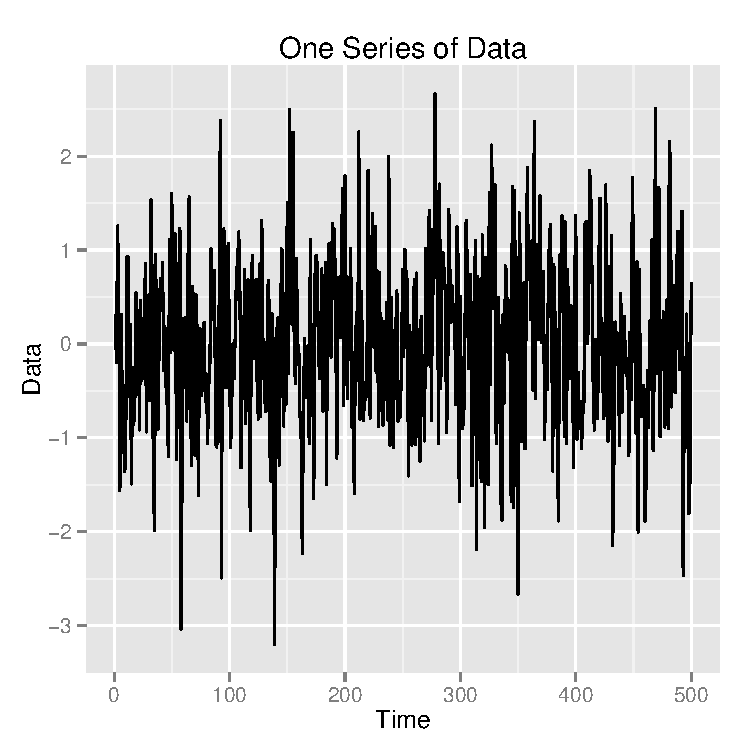
\includegraphics[width=.33\textwidth]{figure/inital-iid1} 
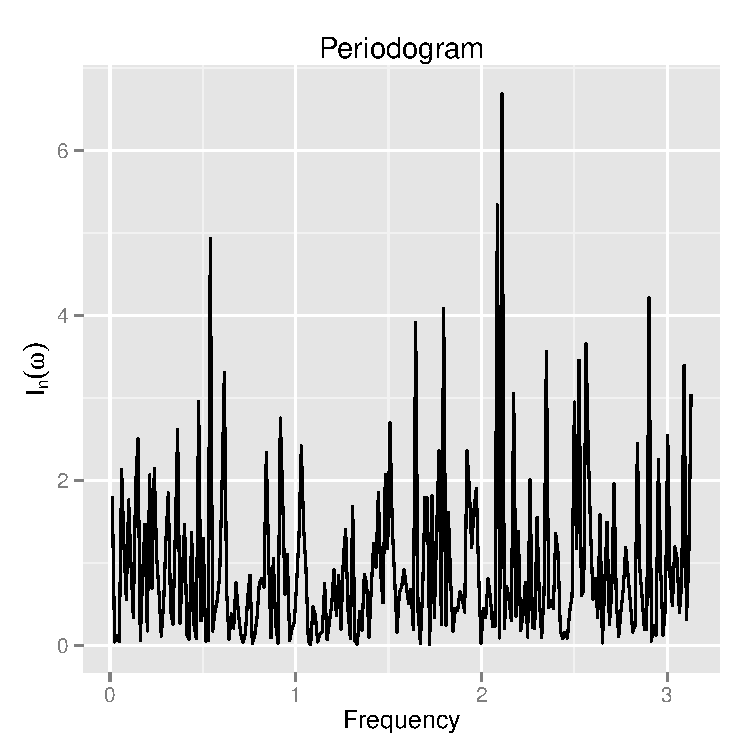
\includegraphics[width=.33\textwidth]{figure/inital-iid2} 
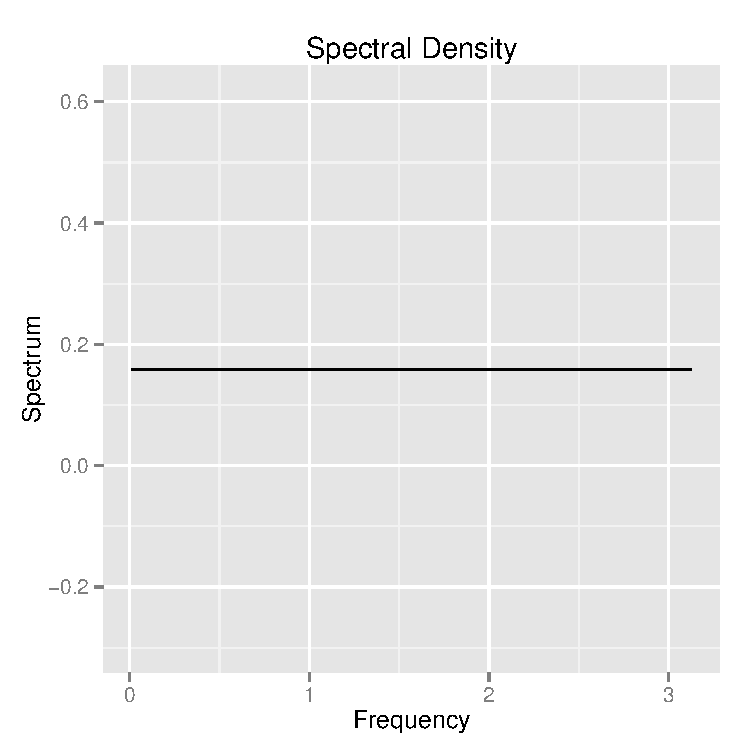
\includegraphics[width=.33\textwidth]{figure/inital-iid3} \caption[One draw, periodogram, and spectral density of a Gaussian IID Model]{One draw, periodogram, and spectral density of a Gaussian IID Model.\label{fig:inital-iid}}
\end{figure}


\end{knitrout}


Tests of exponential distribution and pairwise independence of neighboring Fourier frequencies gave rejection rates relatively similar to the $\alpha$-level of 0.05 over 200 simulations, shown in figure~\ref{fig:tests-iid}. This suggested that the IID Gaussian model results in independent exponentially distributed periodogram ordinates, as expected, and provided some assurance that the testing procedure was performing as expected.

\begin{knitrout}
\definecolor{shadecolor}{rgb}{0.969, 0.969, 0.969}\color{fgcolor}\begin{figure}[h]

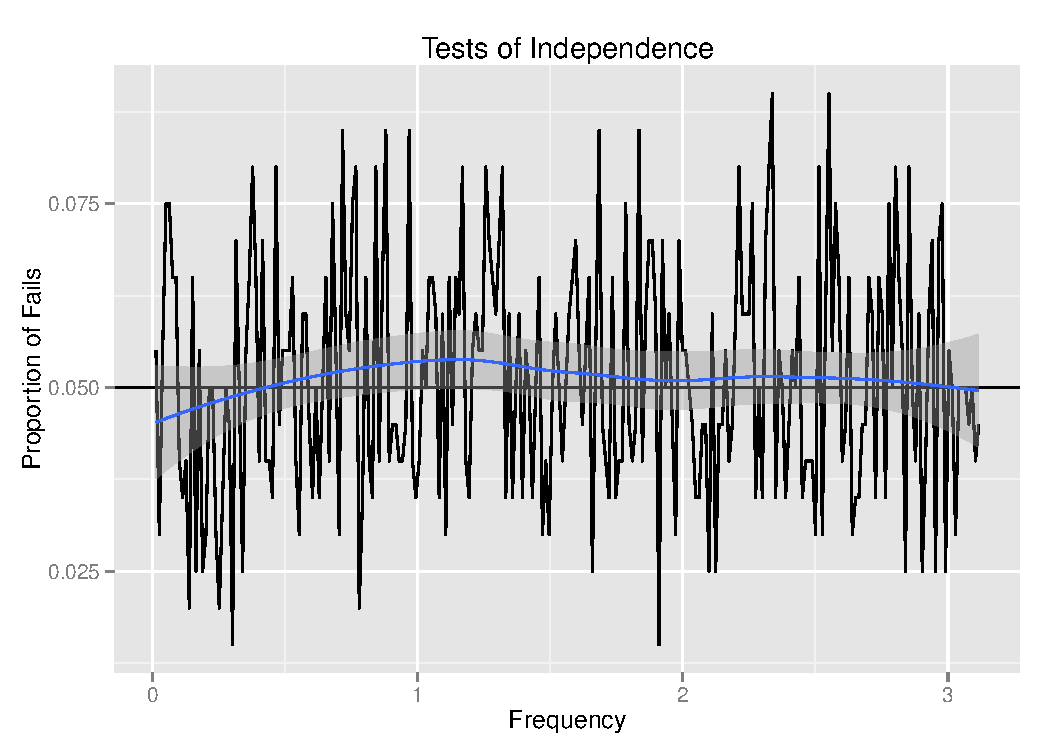
\includegraphics[width=.49\textwidth]{figure/tests-iid1} 
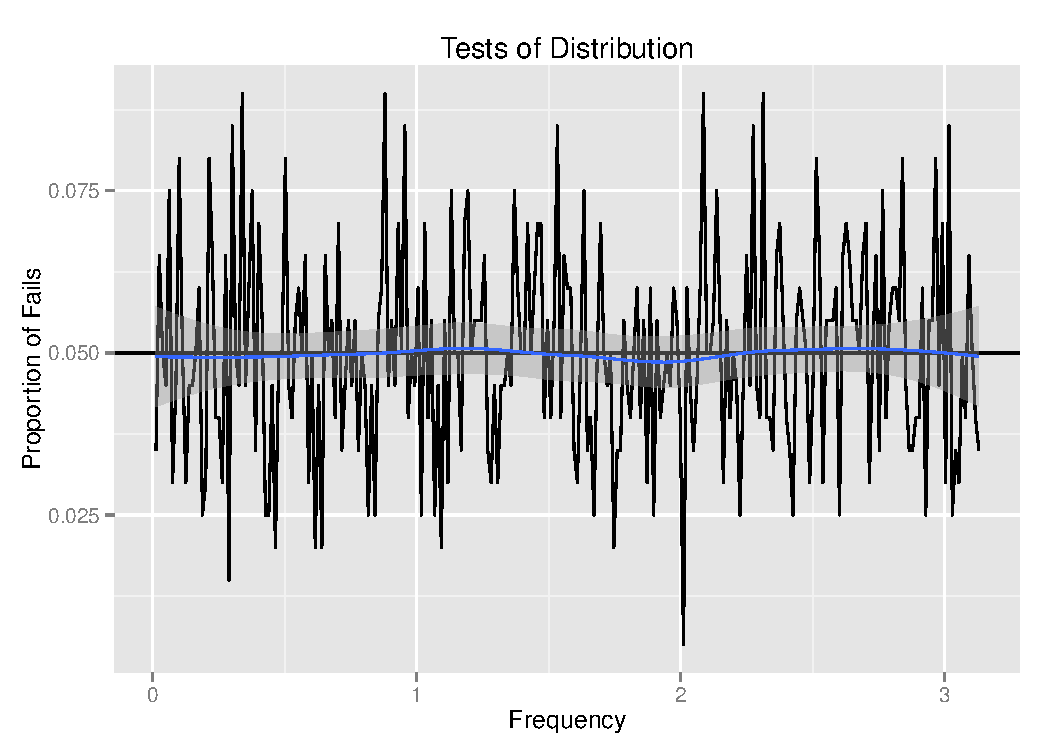
\includegraphics[width=.49\textwidth]{figure/tests-iid2} \caption[Tests of independence and distribution for a Gaussian IID Model]{Tests of independence and distribution for a Gaussian IID Model.\label{fig:tests-iid}}
\end{figure}


\end{knitrout}


\subsubsection{AR(1)}
The first model considered to test the asymptotic assumptions in results~\ref{res:first} and~\ref{res:lahiri} was an AR(1) model with $\phi = 0.5$. For a time series $\{X_t\}$, this model has the form
\begin{align}
X_t = \phi X_{t-1} + Z_t
\end{align}
where $Z_t \sim WN(0, \sigma^2)$. Figure~\ref{fig:inital-ar1} shows that the periodogram for this model has more structure than that of the IID Gaussian with frequencies closer to zero showing up as of higher importance than those further from zero. 
\begin{knitrout}
\definecolor{shadecolor}{rgb}{0.969, 0.969, 0.969}\color{fgcolor}\begin{figure}[h]

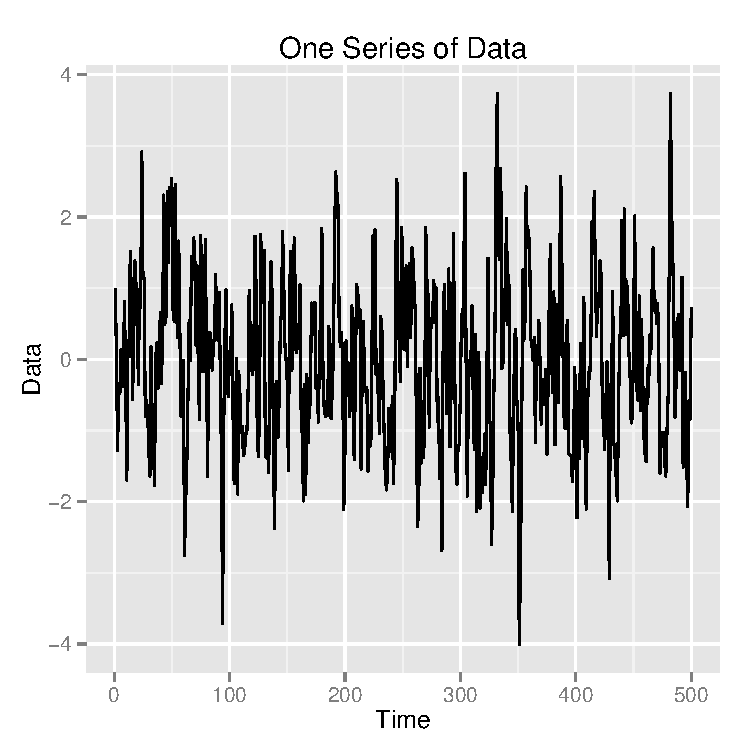
\includegraphics[width=.33\textwidth]{figure/inital-ar11} 
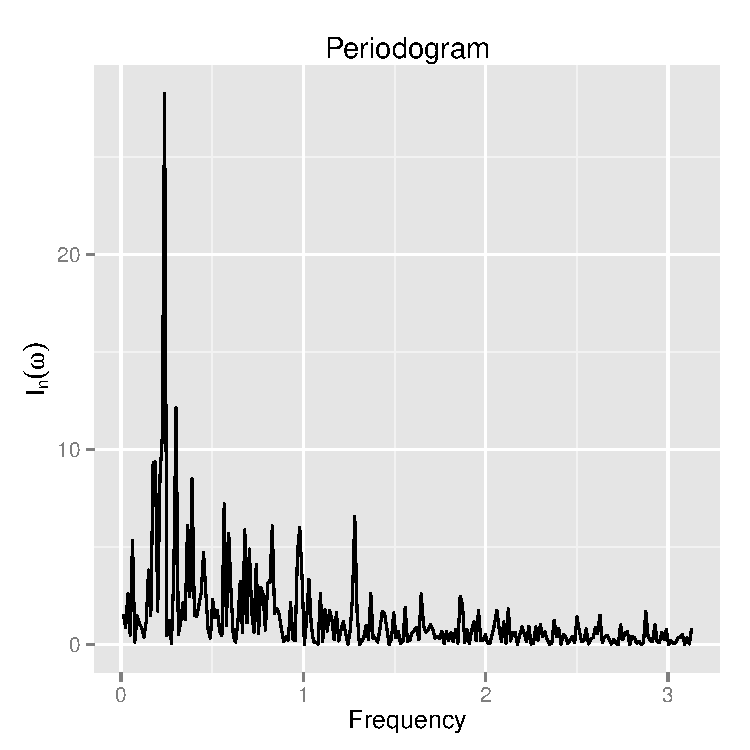
\includegraphics[width=.33\textwidth]{figure/inital-ar12} 
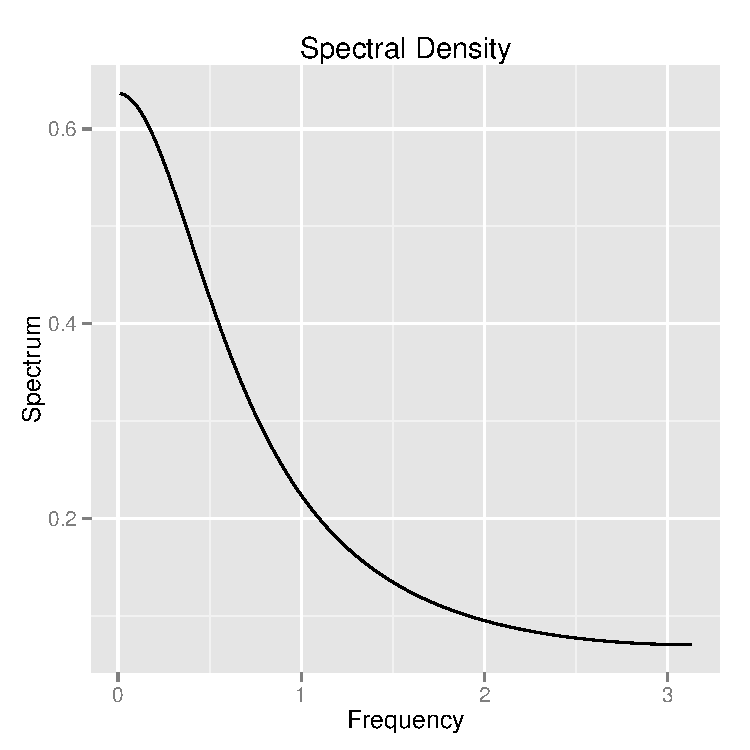
\includegraphics[width=.33\textwidth]{figure/inital-ar13} \caption[One draw, periodogram, and spectral density of an AR(1) model]{One draw, periodogram, and spectral density of an AR(1) model.\label{fig:inital-ar1}}
\end{figure}


\end{knitrout}


The tests of exponential distributions and pairwise independence also gave rejection results consistent with the Type I error rate. Therefore, there was no indication that result~\ref{res:first} does not hold at the Fourier frequencies for an AR(1) model with $\phi=0.5$. This was not entirely surprising as an AR(1) model has only slightly more structure than a white noise model as it represents dependence between neighboring time points only.

\begin{knitrout}
\definecolor{shadecolor}{rgb}{0.969, 0.969, 0.969}\color{fgcolor}\begin{figure}[h]

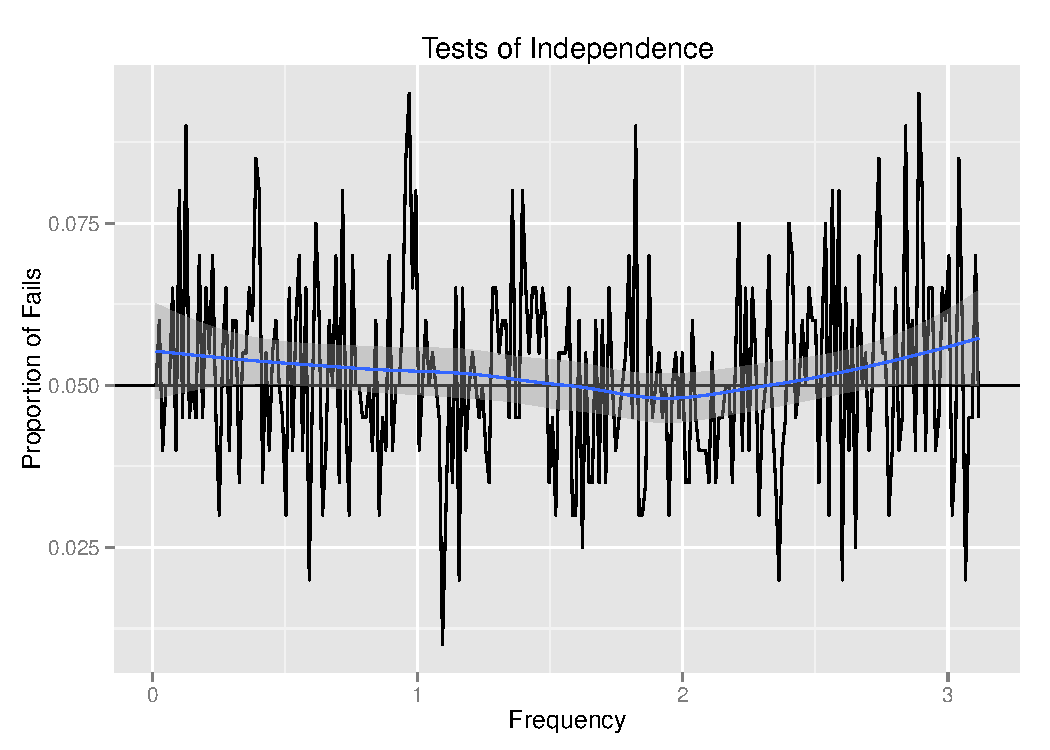
\includegraphics[width=.49\textwidth]{figure/tests-ar11} 
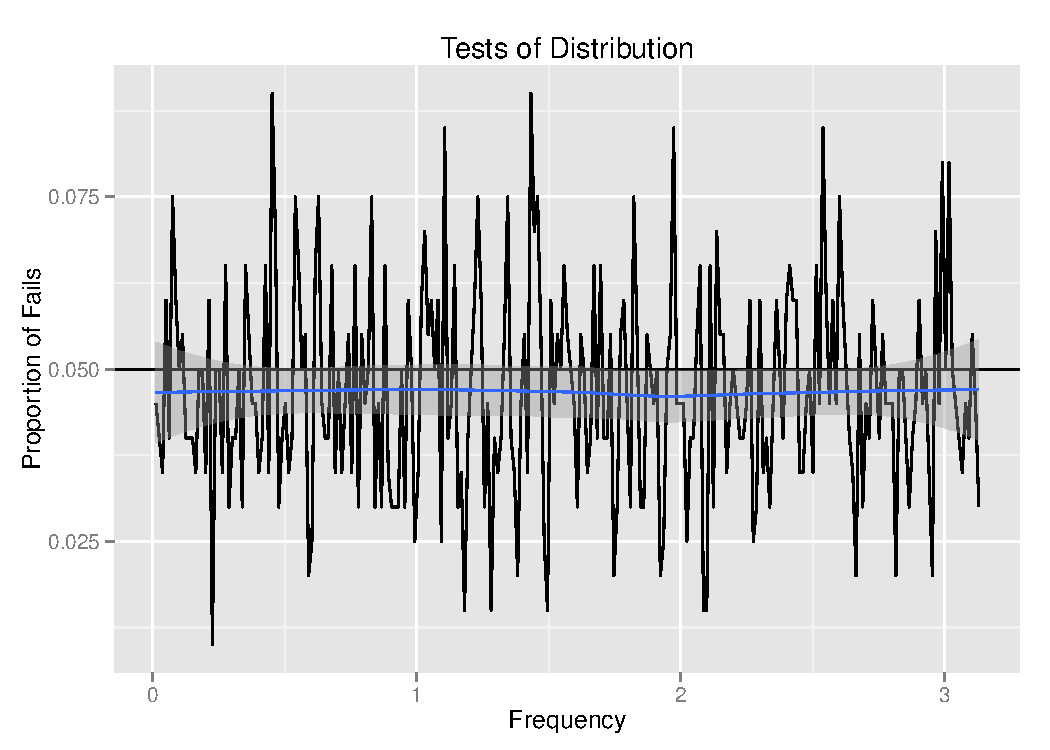
\includegraphics[width=.49\textwidth]{figure/tests-ar12} \caption[Tests of independence and distribution for an AR(1) model]{Tests of independence and distribution for an AR(1) model.\label{fig:tests-ar1}}
\end{figure}


\end{knitrout}


\subsubsection{AR(4)}
To experiment with a time series with a more long-term structure, we implemented an AR(4) model with $\boldsymbol{\phi} = [0.08, 0.33, 0.1, 0.45]$. The estimated periodogram, for simulated time series following this model, is dominated by frequencies very close to zero, figure~\ref{fig:inital-ar4}. 
\begin{knitrout}
\definecolor{shadecolor}{rgb}{0.969, 0.969, 0.969}\color{fgcolor}\begin{figure}[h]

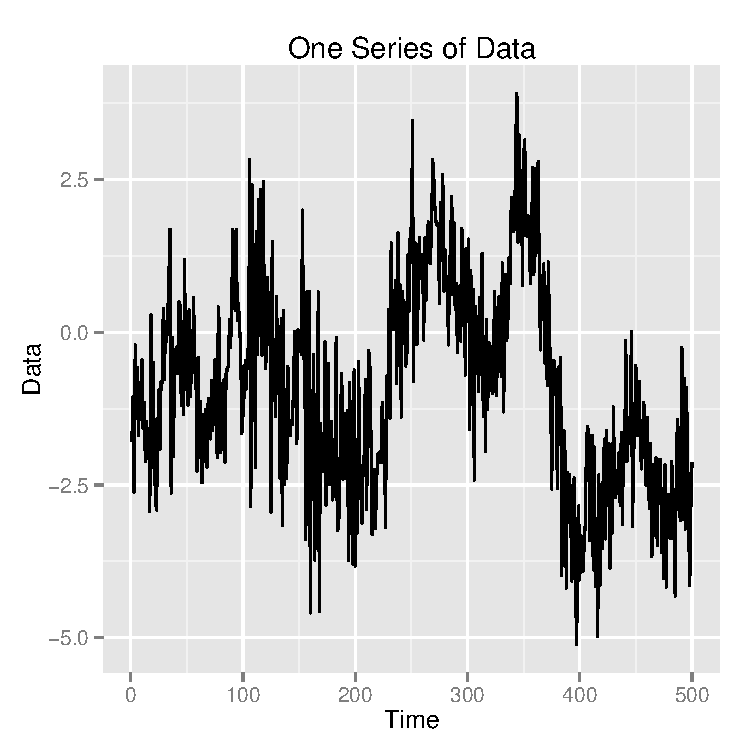
\includegraphics[width=.33\textwidth]{figure/inital-ar41} 
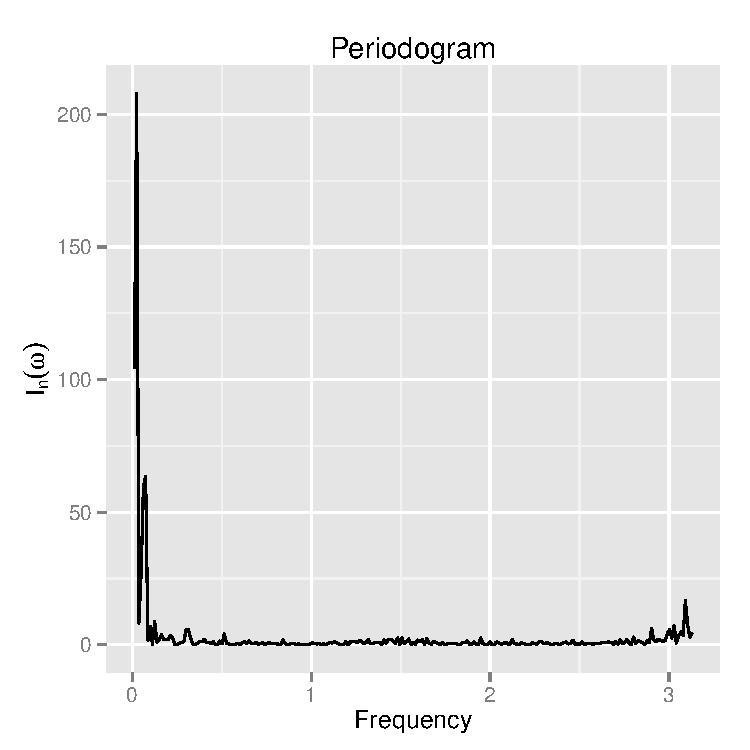
\includegraphics[width=.33\textwidth]{figure/inital-ar42} 
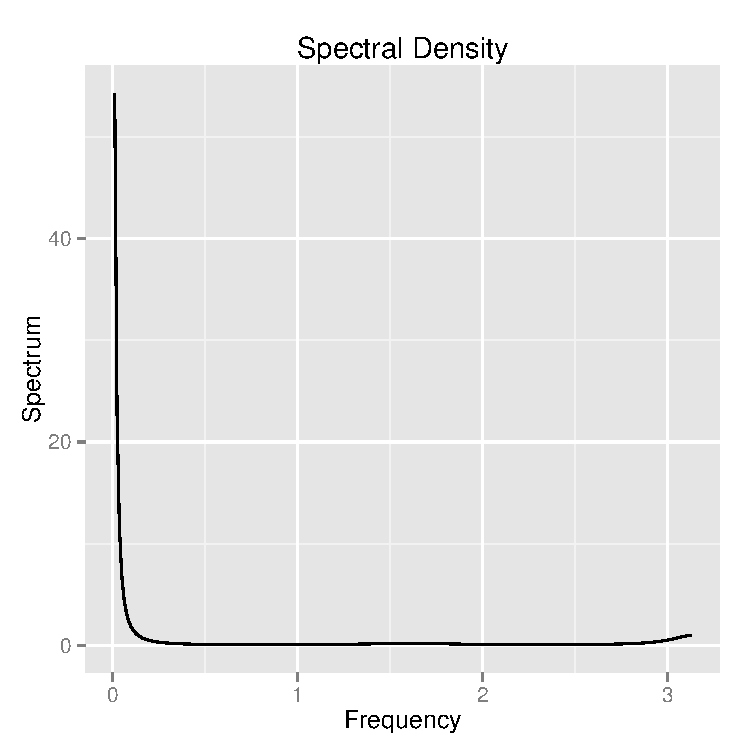
\includegraphics[width=.33\textwidth]{figure/inital-ar43} \caption[One draw, periodogram, and spectral density of an AR(4) model]{One draw, periodogram, and spectral density of an AR(4) model.\label{fig:inital-ar4}}
\end{figure}


\end{knitrout}


Unlike the IID Gaussian and AR(1) models, this AR(4) model does not have rejection rates all similar to $\alpha$ for the independence and exponential tests at neighboring Fourier frequencies. At frequencies closer to zero, the pairwise independence tests fail at rates consistently higher than $\alpha$ and likewise, especially for frequencies less than one, the periodogram ordinates could not be considered to be asymptotically exponentially distributed, see figure~\ref{fig:tests-ar4}. Constructing a sparce subset of Fourier frequencies near zero would not result in asymptotically exponential periodogram ordinates at these frequencies. This is a shortcoming of limiting our method to only looking at differently spaced Fourier frequencies. In this paper, we explore if sparcifying frequencies near zero would satisfy asymptotic independence; see section~\ref{sec:sparce}. Howevever future work could address the question of asymptotic distribution by spacing of non-Fourier frequencies.

\begin{knitrout}
\definecolor{shadecolor}{rgb}{0.969, 0.969, 0.969}\color{fgcolor}\begin{figure}[h]

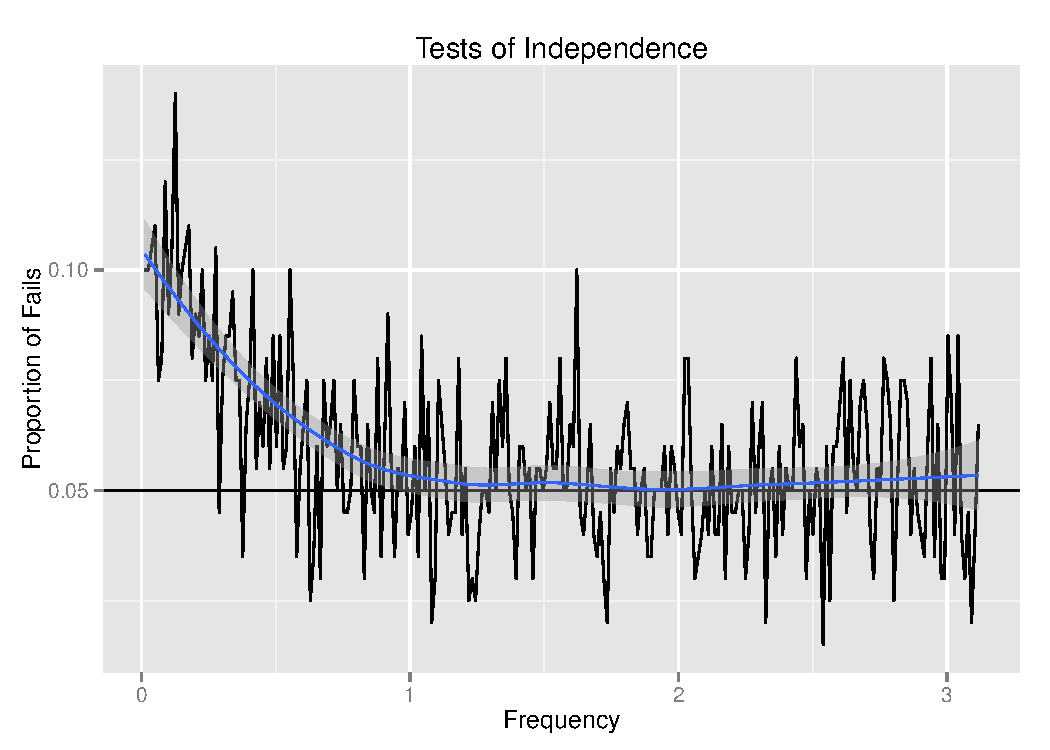
\includegraphics[width=.49\textwidth]{figure/tests-ar41} 
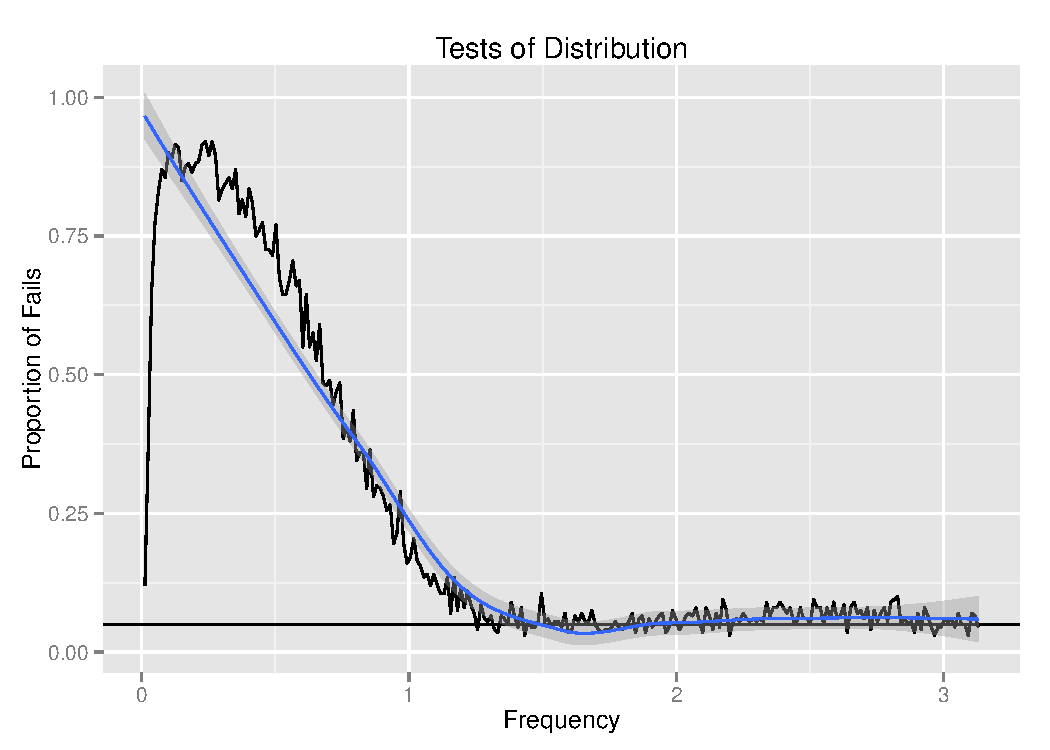
\includegraphics[width=.49\textwidth]{figure/tests-ar42} \caption[Tests of independence and distribution for an AR(4) model]{Tests of independence and distribution for an AR(4) model.\label{fig:tests-ar4}}
\end{figure}


\end{knitrout}


\subsubsection{MA(1)}
We also considered models with moving average structure such as a MA(1) model with $\theta = 0.7$. A time series with this behavior has the form 
\begin{align}
X_t = Z_t + \theta Z_{t-1}
\end{align}
where $Z_t \sim WN(0,\sigma^2)$. Figure~\ref{fig:inital-ma1} shows that the estimated periodogram for a simulated time series of this form puts more importance on frequencies closer to zero than to $\pi$, as in the AR(1) model, but shows a more random structure than the AR(1).
\begin{knitrout}
\definecolor{shadecolor}{rgb}{0.969, 0.969, 0.969}\color{fgcolor}\begin{figure}[h]

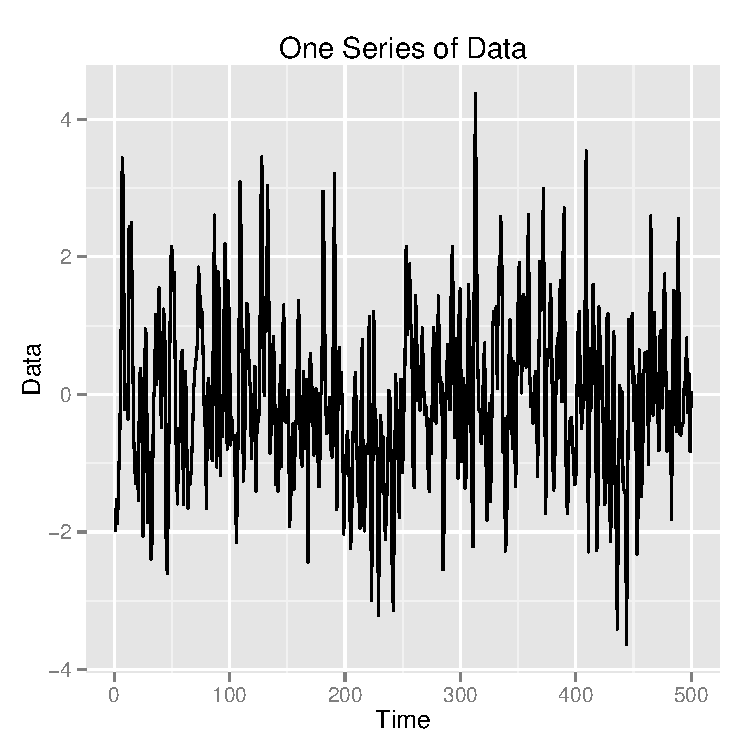
\includegraphics[width=.33\textwidth]{figure/inital-ma11} 
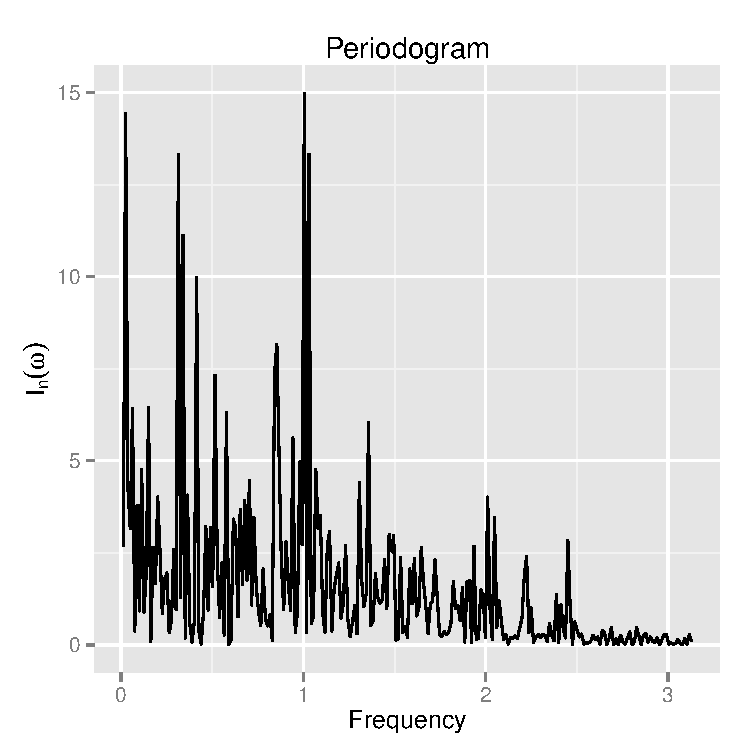
\includegraphics[width=.33\textwidth]{figure/inital-ma12} 
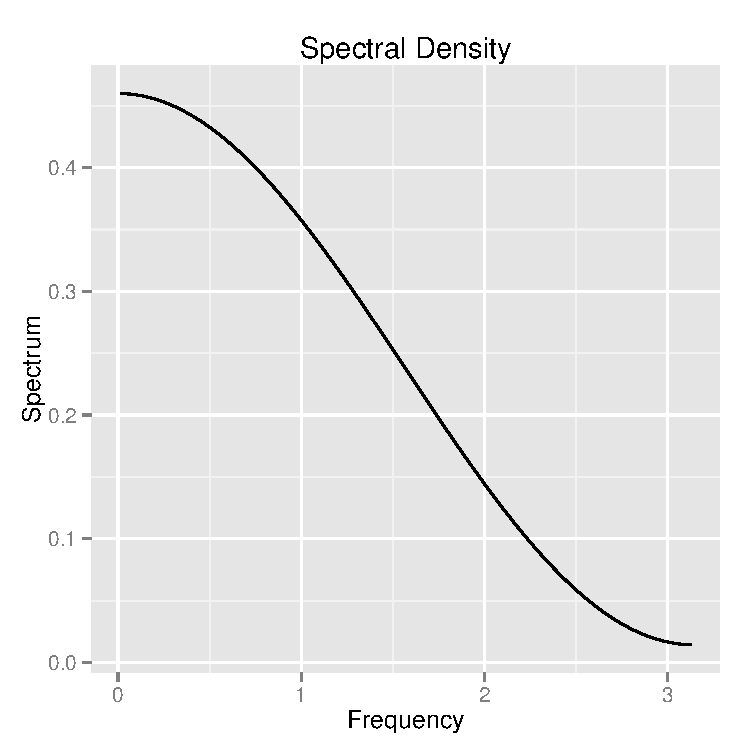
\includegraphics[width=.33\textwidth]{figure/inital-ma13} \caption[One draw, periodogram, and spectral density of an MA(1) model]{One draw, periodogram, and spectral density of an MA(1) model.\label{fig:inital-ma1}}
\end{figure}


\end{knitrout}


The tests of independence gave relatively similar rejection rates to $\alpha$, (figure~\ref{fig:tests-ma1}) indicating no serious departure from pairwise independence at the neighboring Fourier frequencies. The Kolmogorov-Smirnov test gave reasonable rejection rates except for frequencies nearing $\pi$. This was the opposite of what was seen with the AR(4) model, and as sparcifying the Fourier frequencies would not result in asymptotically independent exponentially distributed periodogram ordinates at the these frequencies, the Fourier frequencies nearing $\pi$ would need to be excluded. These frequencies did not appear to be as important in the periodogram in figure~\ref{fig:inital-ma1}, so it could be reasonable to proceed with a subset of frequencies of this type to use in Bayesian modeling of the spectral density. 

\begin{knitrout}
\definecolor{shadecolor}{rgb}{0.969, 0.969, 0.969}\color{fgcolor}\begin{figure}[h]

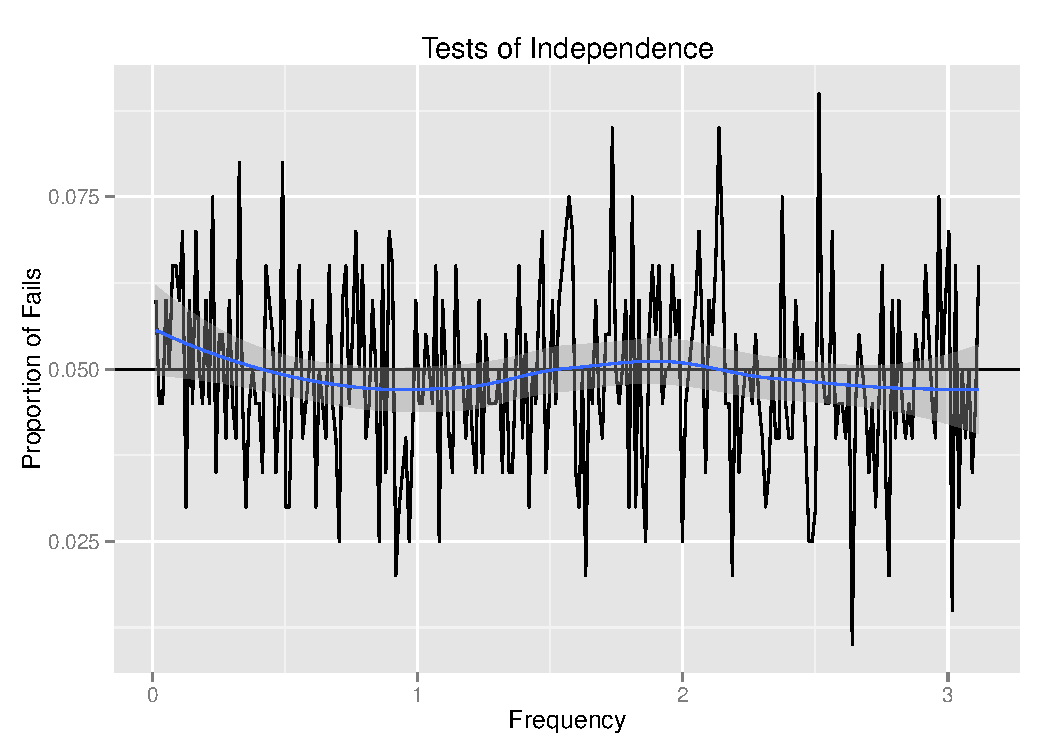
\includegraphics[width=.49\textwidth]{figure/tests-ma11} 
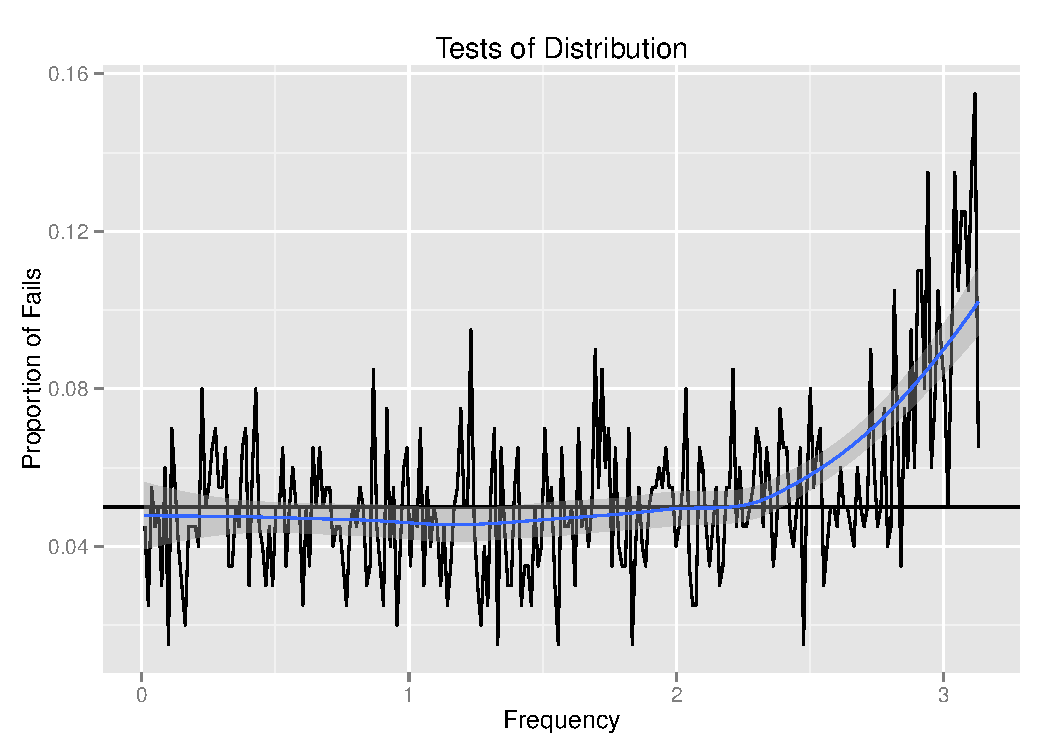
\includegraphics[width=.49\textwidth]{figure/tests-ma12} \caption[Tests of independence and distribution for an MA(1) model]{Tests of independence and distribution for an MA(1) model.\label{fig:tests-ma1}}
\end{figure}


\end{knitrout}


% \subsubsection{MA(2)}
% <<inital-ma2, echo=FALSE, fig.show='hold', fig.width=5, fig.height=5, out.width='.33\\textwidth', fig.cap='One draw, periodogram, and spectral density of an MA(2) model.', fig.pos='h'>>=
% g_draws.ma2
% g_perio.ma2
% g_spec.ma2
% @
% 
% <<tests-ma2, echo=FALSE, fig.show='hold', fig.width=7, fig.height=5, out.width='.49\\textwidth', fig.cap='Tests of independence and distribution for an MA(2) model.', fig.pos='h'>>=
% g_ind.ma2
% g_exp.ma2
% @
% 
\subsubsection{ARMA(4,1)}
Lastly, we considered an ARMA model with both autoregressive (AR) and moving average (MA) components. A time series with this behavior has the form 
\begin{align}
X_t = \phi_1 X_{t-1} + \phi_2 X_{t-2} + \phi_3 X_{t-3} + \phi_4 X_{t-4} + Z_t + \theta Z_{t-1}
\end{align}
where $Z_t \sim WN(0,\sigma^2)$. Specifically, we used the AR and MA coefficients equal to those of the AR(4) and MA(1) models discussed previously.  
\begin{knitrout}
\definecolor{shadecolor}{rgb}{0.969, 0.969, 0.969}\color{fgcolor}\begin{figure}[h]

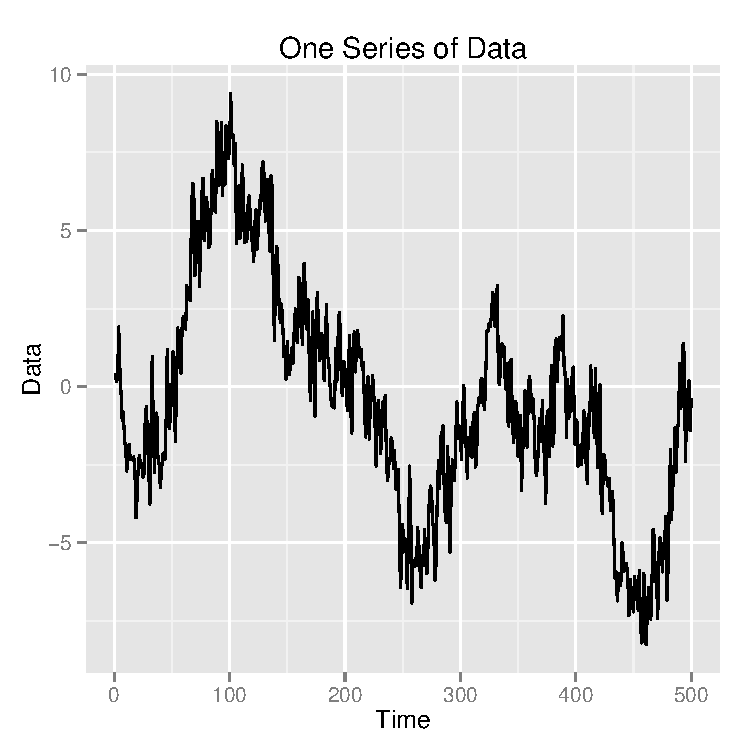
\includegraphics[width=.33\textwidth]{figure/inital-arma411} 
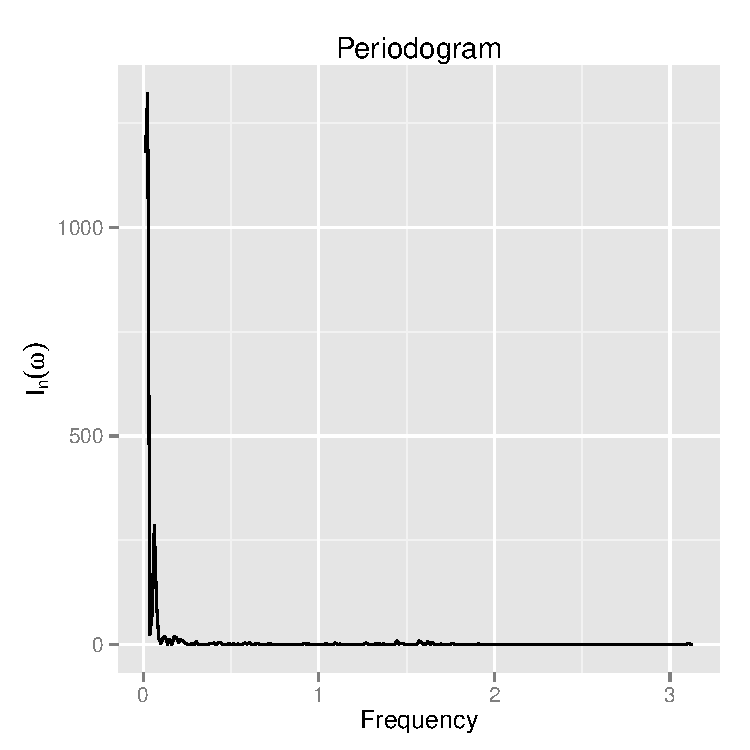
\includegraphics[width=.33\textwidth]{figure/inital-arma412} 
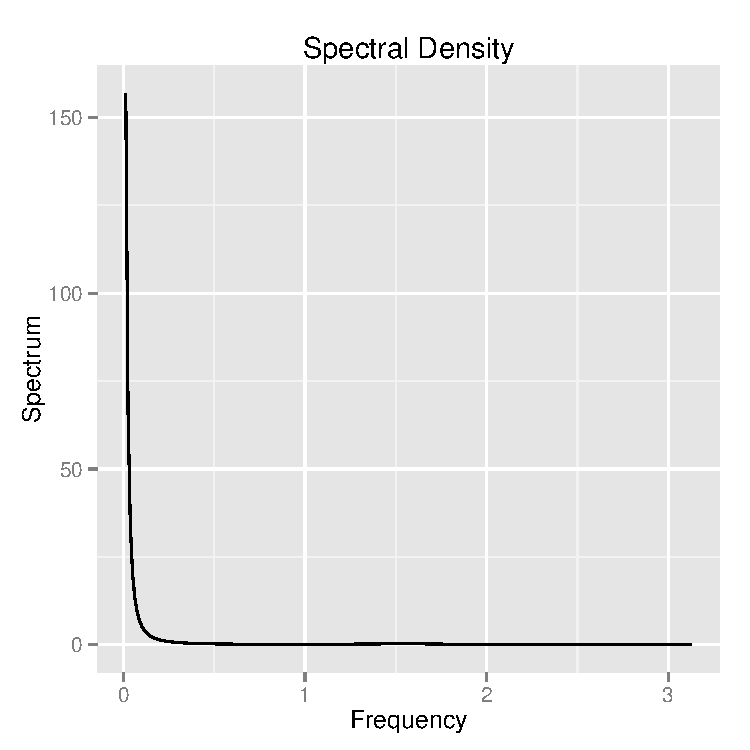
\includegraphics[width=.33\textwidth]{figure/inital-arma413} \caption[One draw, periodogram, and spectral density of an ARMA(4,1) model]{One draw, periodogram, and spectral density of an ARMA(4,1) model.\label{fig:inital-arma41}}
\end{figure}


\end{knitrout}


This ARMA model failed the pairwise Spearman rank correlation tests at frequencies close to zero, in a similar fashion as the AR(4) model. An attempt at sparcifying frequencies close to zero could be made to satisfy the independence conditions of Lahiri~\ref{res:lahiri}. However, the asymptotic exponential assumption is violated at the majority of the Fourier frequencies, as seen in figure~\ref{fig:tests-arma41}. The combination of similar results from the AR(4) at frequencies near to zero and failures at frequences near to $\pi$ from the the MA(1) model result in the ARMA(4,1) satisfying asymptotic exponential distributional properties only at frequencies near $\pi/2$. Once again, this issue can not be resolved by our proposed method and would need to be explored at non-Fourier frequencies.

\begin{knitrout}
\definecolor{shadecolor}{rgb}{0.969, 0.969, 0.969}\color{fgcolor}\begin{figure}[h]

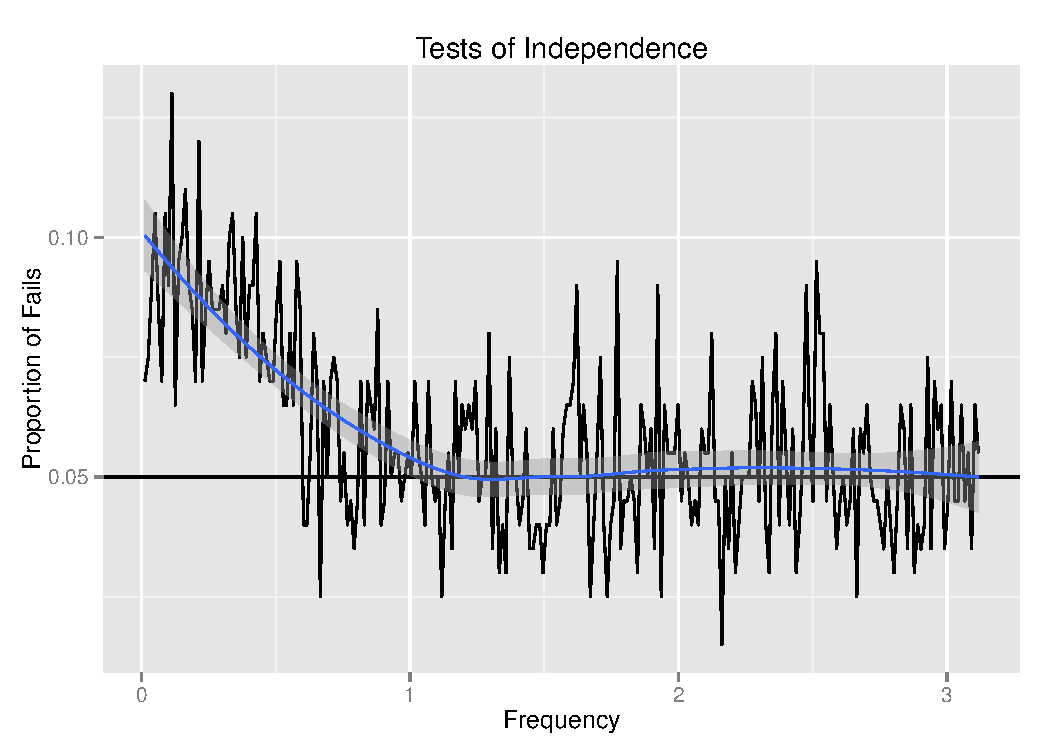
\includegraphics[width=.49\textwidth]{figure/tests-arma411} 
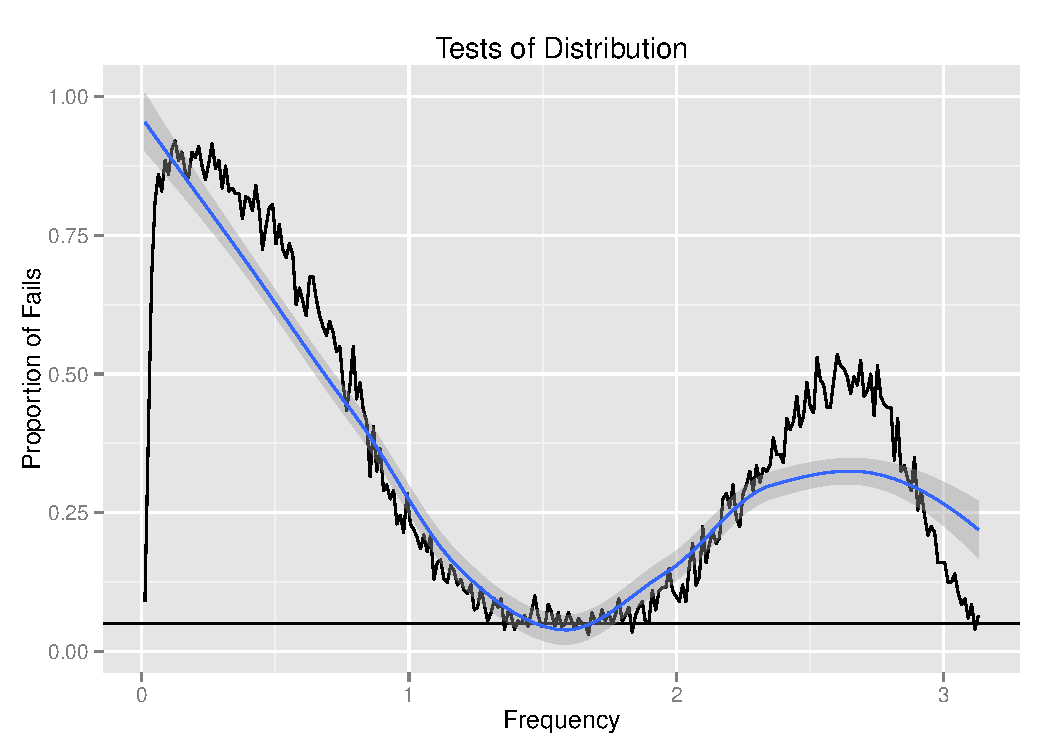
\includegraphics[width=.49\textwidth]{figure/tests-arma412} \caption[Tests of independence and distribution for an ARMA(4,1) model]{Tests of independence and distribution for an ARMA(4,1) model.\label{fig:tests-arma41}}
\end{figure}


\end{knitrout}


% \subsubsection{ARMA(4,2)}
% <<inital-arma42, echo=FALSE, fig.show='hold', fig.width=5, fig.height=5, out.width='.33\\textwidth', fig.cap='One draw, periodogram, and spectral density of an ARMA(4,2) model.', fig.pos='h'>>=
% g_draws.arma42
% g_perio.arma42
% g_spec.arma42
% @
% 
% <<tests-arma42, echo=FALSE, fig.show='hold', fig.width=7, fig.height=5, out.width='.49\\textwidth', fig.cap='Tests of independence and distribution for an ARMA(4,2) model.', fig.pos='h'>>=
% g_ind.arma42
% g_exp.arma42
% @

\subsection{Sparce Frequencies for AR(4)} \label{sec:sparce}
Lahiri's result~\ref{res:lahiri} suggests that, for sparce frequencies and dense frequencies distant from zero, asymptotic independence should hold. We attempted to apply this concept to the AR(4) model to see if we could find a subset where pairwise independence would hold at all frequencies. In figure~\ref{fig:tests-ar4}, asymptotic independence appeared to be satisfied at frequencies roughly larger than $2 \pi*60/500$.  Therefore, we retained all the Fourier frequencies greater than $2 \pi*60/500$ and focused on evenly spaced subsets of frequencies from $2\pi/500$ to $2\pi*60/500$. We considered all possible subsets of Fourier frequencies from $2\pi/500$ to $2\pi* 60/500$ and tested the pairwise independence for each. Choice of starting frequency for each subset was also considered. For example, removing every other frequency would result in two possible subsets, one beginning at $2\pi/500$, the other at $2\pi*2/500$. Examples of spacing frequencies by one (keep every other frequency) subsets and spacing frequencies by two (keep every third frequency) subsets and the rejection rates for pairwise tests of independence are shown in figures~\ref{fig:space1-ar4} and~\ref{fig:space2-ar4}.

\begin{knitrout}
\definecolor{shadecolor}{rgb}{0.969, 0.969, 0.969}\color{fgcolor}\begin{figure}[h]

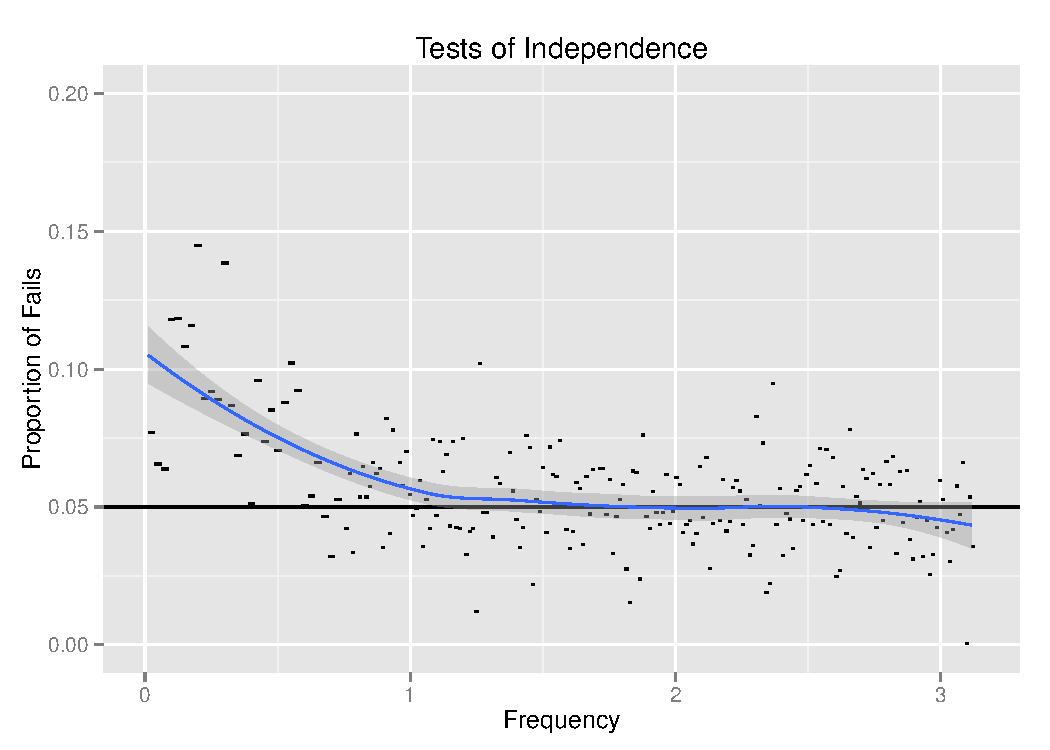
\includegraphics[width=.49\textwidth]{figure/space1-ar41} 
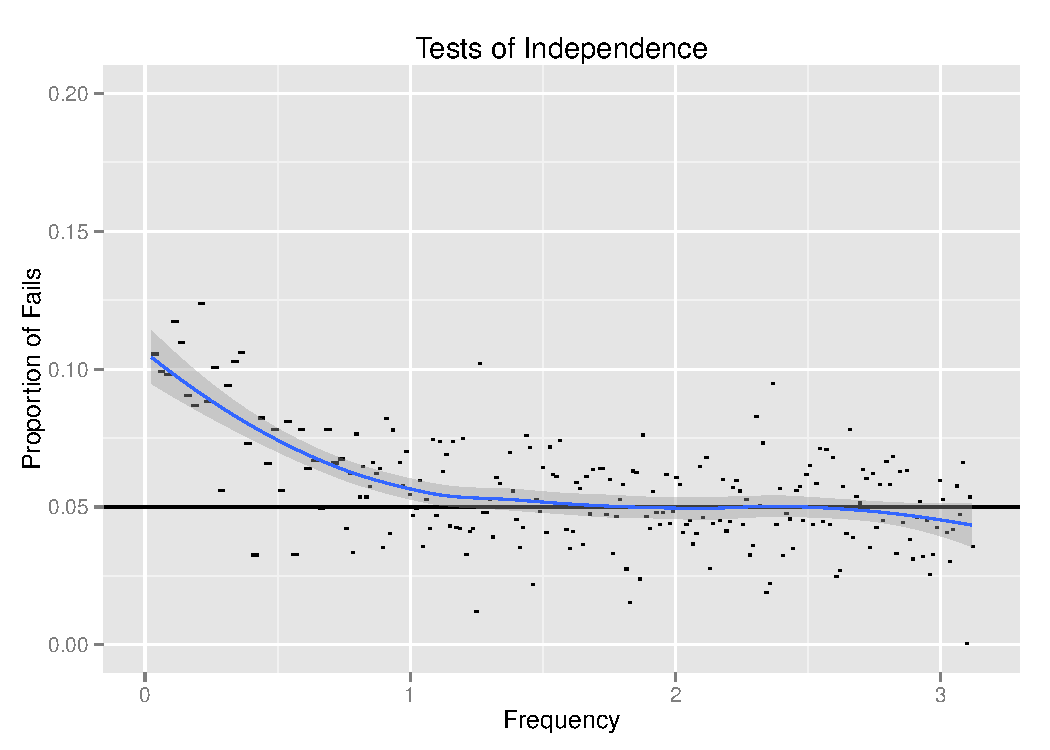
\includegraphics[width=.49\textwidth]{figure/space1-ar42} \caption[Tests of pairwise independence for every other Fourier frequency starting at the first and second Fourier frequencies, respectively, including the remaining full set of Fourier frequencies]{Tests of pairwise independence for every other Fourier frequency starting at the first and second Fourier frequencies, respectively, including the remaining full set of Fourier frequencies.\label{fig:space1-ar4}}
\end{figure}


\end{knitrout}


\begin{knitrout}
\definecolor{shadecolor}{rgb}{0.969, 0.969, 0.969}\color{fgcolor}\begin{figure}[h]

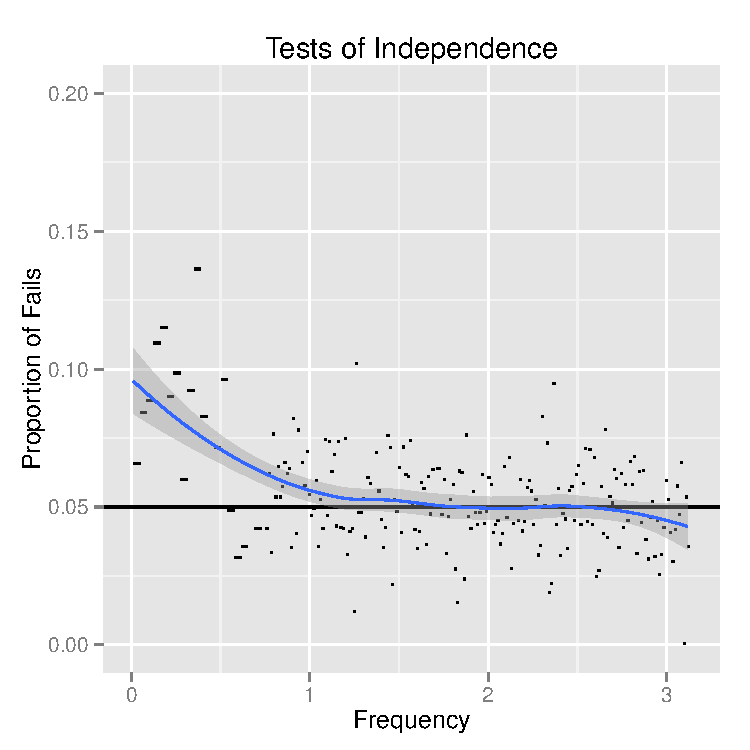
\includegraphics[width=.33\textwidth]{figure/space2-ar41} 
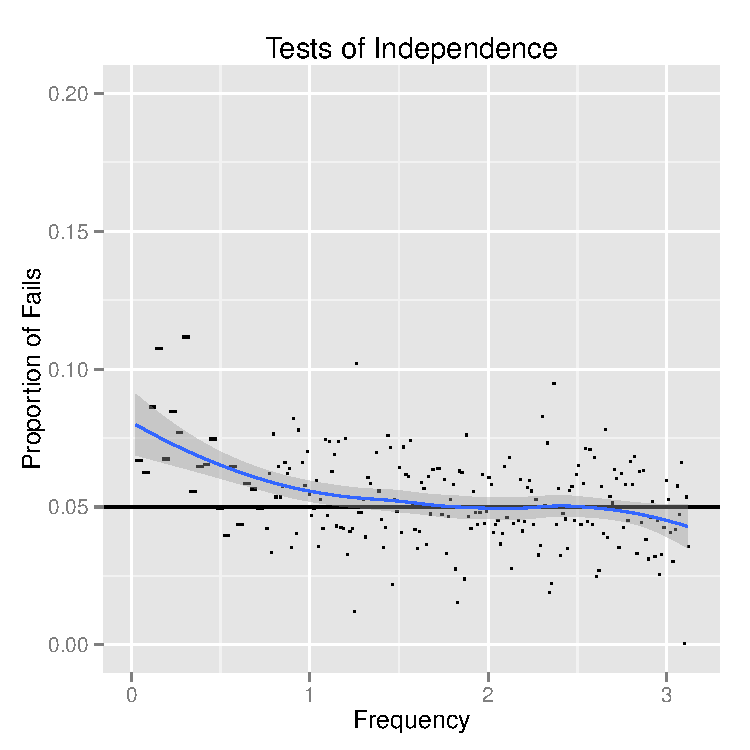
\includegraphics[width=.33\textwidth]{figure/space2-ar42} 
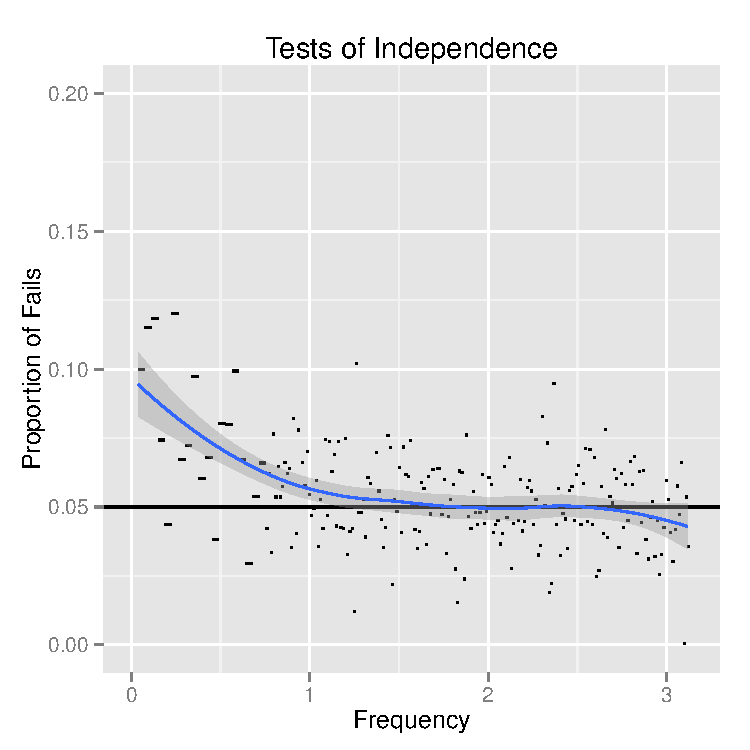
\includegraphics[width=.33\textwidth]{figure/space2-ar43} \caption[Tests of pairwise independence for every third Fourier frequency starting at the first, second and third Fourier frequencies, respectively,including the remaining full set of Fourier frequencies]{Tests of pairwise independence for every third Fourier frequency starting at the first, second and third Fourier frequencies, respectively,including the remaining full set of Fourier frequencies.\label{fig:space2-ar4}}
\end{figure}


\end{knitrout}


The pairwise rejection rates for the subsets shown in figures~\ref{fig:space1-ar4} and~\ref{fig:space2-ar4} decrease slightly from that in figure~\ref{fig:tests-ar4} but still show higher rejection rates than the $\alpha$-level of 0.05. It could be argued that for frequencies roughly greater than $2\pi * 30/500$ in the second subset of every other spacings shown in figure~\ref{fig:space1-ar4}, the asymptotic independence assumption holds. However, considering all other possible spacings between frequencies, we were unable to find a subset that resulted in pairwise independence at frequencies less that $2\pi * 30/500$. This could indicate that frequencies greater than $2 \pi * 25/500$ are sufficiently ``distant from zero", satisfying result~\ref{res:lahiri}. Therefore, a subset of Fourier frequencies where the asymptotic independence result would reasonably hold would be $\{\omega_j=2\pi j/500, j=30,32,34,...,60\} \cup \{\omega_j=2\pi j/500, j=61,62,...,249\}$. Unfortunately, the estimated periodograms for time series of this AR(4) class are dominated by frequencies very close to 0, figure~\ref{fig:inital-ar4}, so this subset would not be practical for a Bayesian analysis, or any analysis of the spectral density. 


\section{Discussion}

This research focused on assessing asymptotic independence and exponential distributional assumptions of periodograms at the Fourier frequencies. In models where asymptotic pairwise independence did not hold at all of the frequencies, we explored the possibility of constructing a subset of frequencies where the asymptotic independence of result~\ref{res:lahiri} was satisfied. In all of the ARMA models we considered, including those discussed, we were either unable to find a lack of pairwise independence at the full Fourier frequencies, or if independence was not satisfied, we were unable to find a suitable subset of frequencies such that result~\ref{res:lahiri} held without removing a large number of important frequencies. For example, in the AR(4) example, pairwise asymptotic independence was satisfied for a subset of frequencies if those near zero were removed. This was a large number of frequencies, roughly $\{2\pi */500,...,2\pi* 30/500\}$ and happened to be the only frequencies that appeared important in the estimated periodograms. Therefore, this subset of frequencies would be relatively useless if anyone wanted to proceed with further practical analysis.

It should be noted that if a set of random variables are all pairwise independent, this does not imply they are jointly independent. In our tests of asymptotic independence, it is possible that in models in which we found an indication of pairwise asymptotic independence, a higher order dependent structure was still present. The use of pairwise independence tests also presented a multiple comparison issue which we have not accounted for here. To test all possible pairs of Fourier frequencies, $\sum_{i=1}^k (k-1)$ pairwise tests are required where $k=\lfloor\frac{n-1}{2}\rfloor$. A familywise error rate correction such as Bonferroni may be too conservative in this application, so other multiple comparison corrections should be considered if pairwise independence is to be used to assess asymptotic independence of the periodogram.

In this paper we have focused largely on the assumption of asymptotic independence and the results by Lahiri~\ref{res:lahiri}. However, the asymptotic exponential assumption is equally as important if one were to implement a Bayesian analysis of the spectral density. If our tests of distribution failed at one or more frequencies, the subset of Fourier frequencies that could produce asymptotically independent exponential periodogram ordinates could not include these frequencies. In models such as the MA(2) and ARMA(4,1) we considered, this was a very large number of frequencies and therefore, using the Fourier frequencies for these specific models in a Bayesian analysis would be incredibly ineffective. In order to address the issue of asymptotic exponential distributions, we could examine spacings of non-Fourier frequencies near zero. However, the benefit of this option has not been explored.

Additionally, our research focused only on stationary ARMA time series due to the known closed-form of the spectral density function in these models. It should be noted that in more interesting cases, i.e. models with a seasonal structure, these models do not have known closed-form spectral densities, and thus we were unable to include them in this research. This is because without the values of the spectral density at tested frequencies, we would be unable to use the KS test for distributional fit. There are two alternatives that can be visited in future work. The first is using an unbiased and consistent estimator of the spectral density (like a window estimator \cite{brockwell2002introduction}) as the mean of the scaled periodogram. A sensitivity analysis could be conducted to determine bandwidth. The second is to use a modification of the KS test called the Lilliefors test for the exponential distribution. This test is designed to test the null hyptothesis, $H_0: \text{The random sample has the exponential distribution with unknown mean}$, against the alternative hypothesis, $H_1: \text{The distribution is not exponential}$ \cite{conover1998practical}. At the time of this writing, the Lilliefors test is not implemented in R. Through the use of one of these modifications, it may be possible to apply this method to models with a more general structure.

As a final note, in our experience the spacings of frequencies depended strongly on what model the data was generated from. In practice, one will never know what process underlies the data (thus a model fitting procedure is employed). Because of this, the spacing procedure will not be generalizable across multiple models. Furthermore, this method is impossible to employ in a live situation even with the modifications mentioned above because one will never have thousands of realizations of their data to check approximate exponential distribution and independence between frequencies of the periodograms.


\printbibliography

\end{document}
